
%\usepackage{booktabs}
%\usepackage{textcomp}
%%\usepackage{color}
%%\usepackage{epstopdf}

\documentclass[10pt]{beamer}
%\usepackage[italian]{babel}
\usepackage[USenglish,british,american,australian,english]{babel}
%\usepackage[latin1]{inputenc}
\usepackage[utf8]{inputenc}
\usepackage[T1]{fontenc}
\usepackage{tikz}
\usepackage{bm} % per avere formule in grassetto
%\usepackage[dvips]{graphicx}

\usepackage{xcolor} % formule o testo a colori
\usepackage{indentfirst}
\usepackage{fancyhdr}
\usepackage{fancybox}
\usepackage{graphicx}
%------librerie matematiche-----
\usepackage{amssymb}
\usepackage{amsmath} 
\usepackage{latexsym}
\usepackage{amsthm} 
\usepackage{eucal} 
\usepackage{eufrak}
\usepackage{enumerate}
\usepackage{subfigure}

% to define colors

\definecolor{remivert}{RGB}{0,160,0}

%--------NEWCOMMAND----

%-- shortcuts for greek letters

\newcommand\eps{\varepsilon}
\newcommand\ph{\varphi}
\newcommand\ka{\kappa}

%\newcommand{\sgn}{sgn}
%\newcommand\ins{}{\{ \}}
%\renewcommand{\ins{}}{\{ \}}
\def \p {{\partial}}
\def \l {{\ell}}

\def \a {{\alpha}}
\def \b {{\beta}}
\def \g {{\gamma}}
\def \d {{\delta}}
\def \la {{\lambda}}
\def \th {{\theta}}

%-- shortcuts for functions
\def \bfA {{\bar{f}^A}}
\def \bfB {{\bar{f}^B}}

\def \hPST {{\hat{\Phi}^{ST}}}
\def \hPAA {{\hat{\Phi}^{AA}}}
\def \hPBB {{\hat{\Phi}^{BB}}}
\def \hPAB {{\hat{\Phi}^{AB}}}
\def \hPBA {{\hat{\Phi}^{BA}}}

\def \PAA {{\Phi^{AA}}}
\def \PBB {{\Phi^{BB}}}
\def \PAB {{\Phi^{AB}}}
\def \PBA {{\Phi^{BA}}}

%-- shortcuts for operators in macro model
\def \Linkop {{\mathcal{L}}}
\def \Difop {{\mathcal{D}}}
\def \Logop {{\mathcal{R}}}

%-- shortcuts fo the parameters of the model
\def \nucST {{\nu_c^{ST}}}
\def \nucAA {{\nu_c^{AA}}}
\def \nucAB {{\nu_c^{AB}}}
\def \nucBA {{\nu_c^{BA}}}
\def \nucBB {{\nu_c^{BB}}}

\def \nudST {{\nu_d^{ST}}}
\def \nudAA {{\nu_d^{AA}}}
\def \nudAB {{\nu_d^{AB}}}
\def \nudBA {{\nu_d^{BA}}}
\def \nudBB {{\nu_d^{BB}}}

\def \KST {{\kappa^{ST}}}
\def \KAA {{\kappa^{AA}}}
\def \KAB {{\kappa^{AB}}}
\def \KBA {{\kappa^{BA}}}
\def \KBB {{\kappa^{BB}}}

%----------------

\theoremstyle{remark}
\newtheorem{remark}{Remark}[section]

% font-size for selected slides
\newcommand\Fontv{\fontsize{7}{7.2}\selectfont}
\newcommand\Fontvi{\fontsize{8}{7.2}\selectfont}
\newcommand\Fontvii{\fontsize{9}{7.2}\selectfont}

% SLIDE 0
%--------------------TITLE PAGE------------------
\title[CEMRACS 2018]{CEMRACS 2018 project:  Mathematical modelling of cell aggregation and segregation.}
%\color{magenta}\shadowbox{Marta Marulli}
%\author[M. Marulli]{Marta Marulli, \\
%\author[1]{Kevin Atsou, Marta Marulli, Rémi Tesson}
%\author[2]{Marta Marulli}
%\author[3]{Rémi Tesson}
%%\author[1]{Static}
%\affil[1]{Laboratoire J.A. Dieudonné, Université de Nice Sophia-Antipolis,}
%\affil[2]{LAGA, Université Paris 13, Università di Bologna,}
%\affil[3]{Institut Mathématiques de Marseille, Aix-Marseille Université}

\author[K.Atsou, M.Marulli, R.Tesson]{Kevin Atsou, \textsuperscript{1} \and Marta Marulli, \inst{2} \and Remi Tesson. \inst{3}}
\institute[]{\textsuperscript{1}  Laboratoire J.A. Dieudonné, Université de Nice Sophia-Antipolis, \and \inst{2} LAGA, Université Paris 13, Università di Bologna, \and \inst{3} Institut Mathématiques de Marseille, Aix-Marseille Université.}



%\textit{in collaboration with}  \\
\date{August 22th 2018}
%\institute{University}
%\logo{\includegraphics[width=15mm]{logo2}}

%------LOGO-----------------------------------------------
\logo{%
  
\includegraphics[width=1.5cm,height=1cm,keepaspectratio]{logo_cirm}}

% beamer theme
\usetheme{Annarbor}
\usecolortheme{lily}

\begin{document}
\begin{frame}
\maketitle
\end{frame}



\section{Introduction}
\begin{frame}
\Fontvii
\frametitle{Biological context}
Cells of the same type can regroup into regions  $\Rightarrow $ spatial organisation. \\
\textbf{Cell segregation} and border sharpening in two-species systems:
\begin{figure}
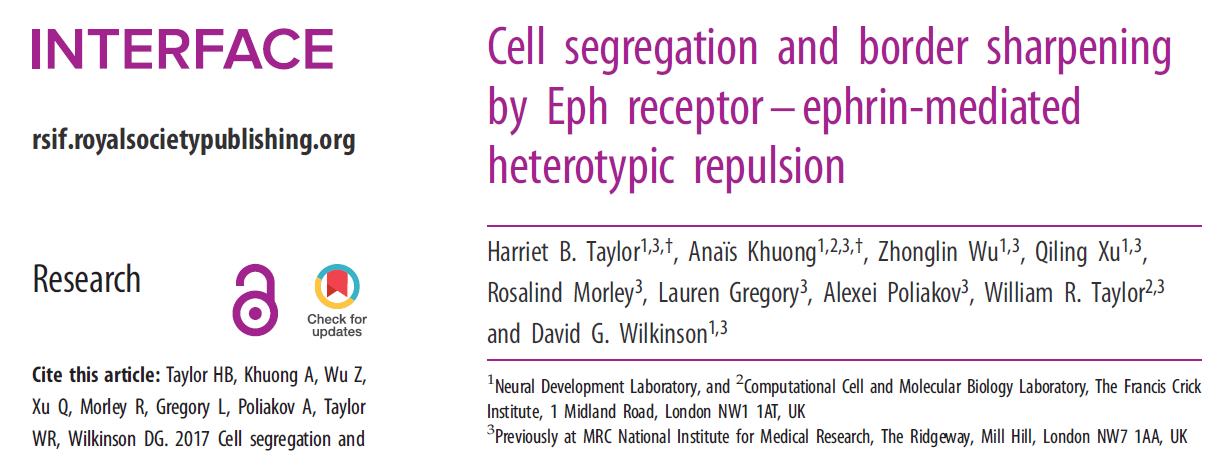
\includegraphics[height=2.5cm, width=9.5cm]{bio_paper}
\end{figure}

\textbf{Working hypothesis:} inter(heterotypic) and intra(homotypic) species repulsion control cell segregation and border sharpening. They have more influence than inter- or intra- species adhesion. 
 
\textbf{Goal:} to understand the mechanisms of morphogenesis.

\begin{figure}[hb]
	\centering
	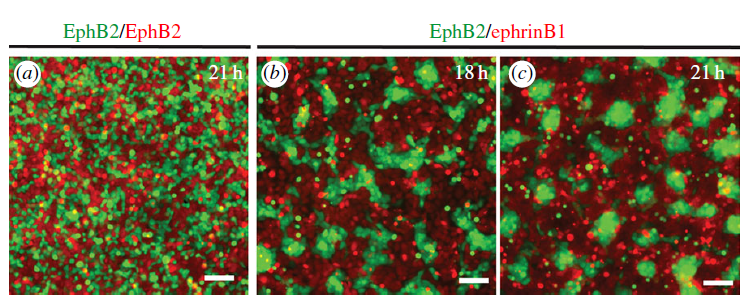
\includegraphics[scale=.45,keepaspectratio]{bio_image}
\end{figure}

\end{frame}


\begin{frame}
\frametitle{How to model?}
Several mathematical models and differents approaches have been proposed for cell segregation. 

\vspace{0.5cm}
\begin{columns}[T] % align columns
	\begin{column}{.48\textwidth}
		\color{blue}\rule{\linewidth}{4pt}
			Macroscopic model	
		\begin{itemize}
			\item Continuous approach $\rightarrow$ analysis tools
			\item Theoretical framework to link the solutions to the model parameters \\
			\vspace{0.5cm}
			BUT
			\item Loss of info about cell-interactions
			\item No info about number of clusters size and popolation size
		\end{itemize}
		
		
	\end{column}%
	\hfill%
	\begin{column}{.48\textwidth}
		\color{blue}\rule{\linewidth}{4pt}
	Microscopic model	
\begin{itemize}
	\item Agent-based models: simplicity and flexibility
	\item Precision of the modeling
	\item Link with experimental data \\
	\vspace{0.5cm}
	BUT
	\item Computational expensive
	\item Theoretically harder
\end{itemize}
		
	\end{column}%
\end{columns}
\end{frame}


\section{Mathematical Model}
\begin{frame}
\frametitle{Microscopic framework}
\Fontvii

\textbf{Individual Based Model} for particles interacting through repulsion interactions:
\begin{equation}
	\begin{cases}
d X_i^{A}=-\mu \nabla_{X_{i}^{A}}W^{A}(X^{A},X^{B})dt + \sqrt{2D_{A}} d B_{i}, \quad \forall i \in\{1, \dots, N_{A}\}
\\
d X_i^{B}=-\mu \nabla_{X_{\l}^{A}}W^{B}(X^{A},X^{B})dt + \sqrt{2D_{B}} d B_{\ell}, \quad \forall \l \in \{1, \dots, N_{B}\}
\end{cases}
\end{equation}
\begin{itemize}
\item $\mu>0$ is the constant mobility coefficient, 
\item  $B_i$ is a 2-dimensional Brownian motion $B_i=(B_i^1,B_i^2)$ of intensity $D_A,D_B>0$ respectively for species A and B,
\item $W^S$ total energy of the S-type particle, $S \in \{ A,B \}$, defined as:  

 $$ W^{A}(X^{A},X^{B})=\underbrace{\sum_{k_1=1}^{K_{AA}} \PAA(X^{A}_{i(k_1)}-X^{A}_{j(k_1)})+
\sum_{k_3=1}^{K_{AB}} \PAB(X^{A}_{i(k_3)}-X^{B}_{\l(k_3)})}_{sum \ over \ all \ pairwise \ link \ potentials \ acting \ on \ particles \ A},  $$

$$ W^{B}(X^{A},X^{B})=\sum_{k_2=1}^{K_{BB}} \PBB(X^{B}_{\l(k_2)}-X^{B}_{m(k_2)})+
\sum_{k_3=1}^{K_{AB}} \PBA(X^{B}_{\l(k_3)}-X^{A}_{\l(k_3)}) $$
%$W^{S}(X^{S},X^{T})=\sum_{i \ne j: |X_i^S-X_j^S|<R} \Phi^{SS}(X_{i}^{S},X_{j}^{s})+ \sum_{i \ne j: |X_i^S-X_j^S|<R}  $

\end{itemize}
\end{frame}


\begin{frame}
\frametitle{Case: Hookean interaction potential}
\Fontvii
We suppose that the homotypic (AA,BB) species links and heterotypic (AB,BA) act as a springs of equilibrium length $R$ between the particles that it is also detection radius  for the interaction.

\begin{tabular}{cl}  
	\begin{tabular}{c}
		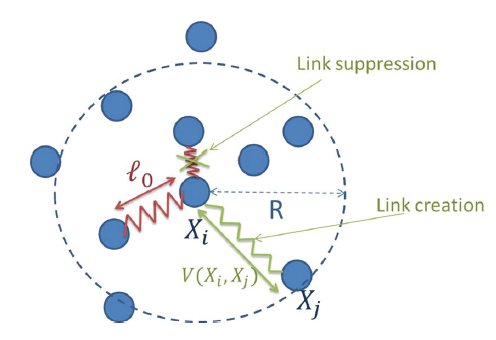
\includegraphics[height=3cm, width=4cm]{link}
	\end{tabular}
	& \begin{tabular}{l}
		\parbox{0.5\linewidth}{%  change the parbox width as appropriate
			\textbf{Case of Hookean springs} \\  
			$$
			\Phi^{ST}(x)=\frac{\nucST}{\nudST}\frac{\KST}{2}
			\begin{cases}
			(|x|-R)^2, \quad \text{for } |x|\leq R\\
			0, \quad \text{for } |x|> R
			\end{cases}
			$$
			with $\nu_{c}^{ST},\nu_{d}^{ST}$ Poisson processes frequencies and $\ka^{ST}$ interaction/repulsion intensity.
		}
	\end{tabular}  \\
\end{tabular}
\vspace{0.5cm}
%Each link is supposed to act as a spring by generating a pairwise potential

\begin{itemize}
	\item[-] Each particle can link/unlink with its neighbors located in a ball of radius $R$
	\item[-] Links are not permanent: created and supressed via random processes 
	\item[-] Linking/unlinking processes are very fast
\end{itemize}
	
\end{frame}


\begin{frame}
\frametitle{Logistic growth term}
%\Fontvii
We add a growth process to the microscopic model as follows:

\begin{itemize}
	\item  Cell of type $S$ divide into 2 cells with probability $\textcolor{blue}{\beta_S}$ and die with probability $\textcolor{remivert}{\delta_S}$ at each time step. $S \in \{ A,B\}$
	%Each individual can give birth to a new one with a probability $\beta$ or die, with a probability $\alpha$. 
	\item  Birth and death processes depend on the local density of individuals
	\item Birth occurs at distance $r$ 
	\end{itemize}
\begin{equation}
\textcolor{blue}{\beta_{S}(X_i) = b_0^{S} -(b_0^{S} - \theta)\left(\frac{\mathcal{N}_{0}}{N^{*}}\right)},
\quad
\textcolor{remivert}{\delta_{S}(X_i) = d_0^{S} + (\theta - d_0^{S}) \left(\frac{\mathcal{N}_{0}}{N^{*}}\right)}
\end{equation}


\textbf{Parameters:}
\begin{itemize}
\item $\mathcal{N}_{0}=\mathcal{N}_{R_0}(X_i^S)$: number of cells (of both population) at distance $R_0$ of the cell located in $X_i^S$ 
\item $N^*$ is the maximal number of cell in a radius $R_0$ allowing cell division. 
\item $\theta$, constant coefficient that assures the randomness at the population $N^{*}$.
%in the range $d_{0}^{S}<\theta<b_{0}^{S}$.

\end{itemize}


\end{frame}



\begin{frame}
\frametitle{Micro macro}

\end{frame}

\begin{frame}{Form micro to macro}{Fock space}
\begin{itemize}
	\item Main difficult the varying size of the cell population
	\item  Introduction of the Fock Space: 
	\item Probability space of all the possible states of the particle system
	$$ X_k := \left[ x_1, x_2, \ldots, x_k \right] $$
	$$ \mathbb{P}_k(X_k,t)dX_k = \text{Pr\{k cells, with one cell in }dx_1,\text{ another in } dx_2\text{ etc. \}} $$
\end{itemize}
\end{frame}

\begin{frame}{Form micro to macro}{Reduced distribution function}
\begin{itemize}
	\item  The density or concentration of cells is define by: 
	$$ f(x,t) = \langle \sum_{p=1}^{k} \delta(x-x_p)\rangle . $$
	which becomes
	$$f(x,t) =  \sum_{k=1}^{\infty} k \int \mathbb{P}_k(x, X_{k-1}, t)dX_{k-1},$$
	\item  We define a master equation for the Probability  $\mathbb{P}_k(X_{k}, t)$ time evolution: 
\end{itemize}
\end{frame}

\begin{frame}{Master Equation}
\begin{align*}
\label{masterEquation}
\mathbb{P}_k(X_k, t+\tau) &= \int \mathbb{W}_k(X_k, t+\tau \vert X_k^{'},t)\mathbb{P}_k( X_k^{'},t)d X_k^{'} \nonumber \\ 
&+ \tau \sum_{i=1}^{k-1}\beta(X_i) \mathbb{B} \mathbb{P}_{k-1} - \tau \left[ \sum_{i=1}^{k} (\beta(X_i) + \delta(X_i)) \right] \mathbb{P}_k(X_k,t) \\ 
&+ \tau \int \sum_{k=1}^{k+1} \beta(X_i) \mathbb{P}{_k+1}(X_{k+1}, t)dx_i \nonumber
\end{align*}
with $\mathbb{W}_k(X_k, t+\tau \vert X_k^{'},t)$ the transition probability from a state $X_k^{'}$ to a state $X_k$ and 
\begin{equation}
\label{birthOperator}
\mathbb{B} \mathbb{P}_{k-1} = \dfrac{2}{k(k-1)} \sum \sum_{1 \leq p < q \leq k} \delta_{pq} \mathbb{P}_{k-1} (X_{k|p},t) 
\end{equation}
\end{frame}

\begin{frame}{Master Equation}
Using Kramers-Moyal expansion on the term $\int \mathbb{W}_k(X_k, t+\tau \vert X_k^{'},t)\mathbb{P}_k( X_k^{'},t)d X_k^{'}$: 
\begin{align*}
\mathbb{P}_k(X_k, t+\tau) &= \left[ 1 + \sum_{\vert \alpha \vert >0} (-1)^{\vert \alpha \vert}  \partial^{\alpha} \left(D^{\vert \alpha \vert} (X_k, t) \tau + O(\tau^2) \right) \right] \mathbb{P}_k(X_k,t) \nonumber \\ 
&+ \tau \sum_{i=1}^{k-1}\beta(X_i) \mathbb{B} \mathbb{P}_{k-1} - \tau \left[ \sum_{i=1}^{k} (\beta(X_i) + \delta(X_i)) \right] \mathbb{P}_k(X_k,t) \\ 
&+ \tau \int \sum_{k=1}^{k+1} \beta(X_i) \mathbb{P}_{k+1}(X_{k+1}, t)dx_i. 
\end{align*}
\end{frame}

\begin{frame}{Master Equation}
the coefficients $D^{\vert \alpha \vert}$ are the so-called\textbf{ Kramers-Moyal} expansion coefficients with:
\begin{equation*}
D^{\vert \alpha \vert} (X_k, t) = \dfrac{1}{\alpha !} \lim_{\tau \rightarrow 0} \dfrac{1}{\tau} \langle (\xi(t+\tau) - X_k)^{\alpha} \rangle \vert_{\xi(t)=X_k}.
\end{equation*}
Using the definition : $$f(x,t) =  \sum_{k=1}^{\infty} k \int \mathbb{P}_k(x, X_{k-1}, t)dX_{k-1},$$
we can deduce the reduced equation on $f(x,t)$ by summing and integrating the master equation. 
\end{frame}


\begin{frame}
\frametitle{Macroscopic framework}
\Fontvii
Macroscopic model should provide an approximation of the agent-based model:
	\begin{equation*}
\begin{cases}
\p_t f^{A}=  \nabla \cdot \underbrace{(f^A\nabla_x(\Phi^{AA}* f^A) + f^A \nabla_x( \Phi^{AB}*f^B))}_{interaction \ potential} + \underbrace{ D_A \Delta_x f^A}_{diffusion} + \underbrace{ \textcolor{red}{\nu_{b}^{A}f^A\left( 1-\frac{f^A+f^B}{f^{*}} \right)}}_{logistic \ term} \\

\p_t f^{B}=  \nabla \cdot (f^B\nabla_x(\Phi^{BB}* f^B) + f^B \nabla_x (\Phi^{BA}*f^A)) + D_B \Delta_x f^B + \textcolor{red}{\nu_{b}^{B}f^B\left( 1-\frac{f^A+f^B}{f^{*}} \right)}
\end{cases}
\end{equation*}
%with  $f^{S}(x,t)$ particle distributions of type S that give the probability to find a particle of type S at a point $x$ and time $t$, $S \in \{ A,B \}$. \\
\begin{itemize}
	\item  $f^*$: carrying capacity of the environment
	\item $\nu_{b}^{A},\nu_{b}^{B}$ growth rates
	%it represents the maximum population size that can be present in the environment.
\end{itemize}
\vspace{0.5cm}

\textcolor{blue}{Remark:}
	$f^{A},f^{B}$ play the same role in logistic term


\end{frame}










\begin{frame}
\frametitle{Analysis of the macroscopic model}
\Fontvi
We recall macroscopic equations for $f^{A}$ and $f^{B}$:
	\begin{equation}
\begin{cases}
\p_t f^{A}=  \nabla \cdot (f^A\nabla_x(\Phi^{AA}* f^A) + f^A \nabla_x( \Phi^{AB}*f^B)) + D_A \Delta_x f^A + \nu_{b}^{A}f^A\left( 1-\frac{f^A+f^B}{f^{*}} \right) \\

\p_t f^{B}=  \nabla \cdot (f^B\nabla_x(\Phi^{BB}* f^B) + f^B \nabla_x (\Phi^{BA}*f^A)) + D_A \Delta_x f^A + \nu_{b}^{B}f^B\left( 1-\frac{f^A+f^B}{f^{*}} \right)
\end{cases}
\end{equation}

Linearization around constant steady states $\bfA, \bfB$ and Fourier transform:
\begin{align*}
\p_t \begin{pmatrix} \hat{f}^A \\ \hat{f}^B
\end{pmatrix}=
\underbrace{\begin{pmatrix} -|y|^2(2\pi\bfA\hPAA(y)+D_A)-\nu_{b}^A\frac{\bfA}{f^*} & -|y|^22\pi\bfA\hPAB(y)-\nu_{b}^A\frac{\bfA}{f^*} \\ 
-|y|^2\bfB\hPBA(y)-\nu_{b}^B\frac{\bfB}{f^*} & -|y|^2(2\pi\bfB\hPBB(y)+D_B)-\nu_{b}^B\frac{\bfB}{f^*} 
\end{pmatrix}}_{M(y)}
\begin{pmatrix} \hat{f}^A \\ \hat{f}^B
\end{pmatrix}
\end{align*}

The constant steady states will be unstable if:
\begin{itemize}
	\item $ \nu^{B}\frac{\bfA}{f^{*}}( \bfA 2\pi \hPAA+D_A - \bfA 2 \pi \hPAB )<
	\nu^{A} \frac{\bfA}{f^{*}}( \bfB 2 \pi \hPBB + D_B-\bfB 2\pi \hPBA ). $	
\end{itemize}
\vspace{0.3cm}
We want to focus on the ratio of homo- and hetero-typic species repulsion. \\
We introduce a parameter $s\in \mathbb{R}$ s.t.: $\textcolor{blue}{\ka^{ST}=s\tilde{\ka}^{ST}} $



%$$s_{L}^{*}=\frac{(24 D_A+c'^{AA})\nu_{b}^{B}\bar{f}^{B}+(24 D_B+c'^{BB})\nu_{b}^{A}\bar{f}^A}{\nu_{b}^{B}\bar{f}^B\tilde{c}'^{AB}+\nu_{b}^{A}\bar{f}^A\tilde{c}'^{BA}}. $$

%\item $ \begin{cases} 
%\nu^{B}\frac{\bfA}{f^{*}}( \bfA 2\pi \hPAA+D_A - \bfA 2 \pi \hPAB )>
%\nu^{A} \frac{\bfA}{f^{*}} ( \bfB 2 \pi \hPBB + D_B-\bfB 2\pi \hPBA ) \\
%|y|^{2}( \bfA 2 \pi \hPAA(y)+D_A )+\nu^A\frac{\bfA}{f^{*}}+|y|^{2}(\bfB 2 \pi \hPBB(y)+D_B )+\nu^{B}\frac{\bfB}{f^{*}} < 0
%\end{cases} $

\end{frame}


\newcommand{\highlight}[1]{%
	\colorbox{yellow}{$\displaystyle#1$}}

\begin{frame}
\frametitle{Analysis of the macroscopic model}
\Fontvii
We find critical value $s_{L}^{*}$ related to instability:
%$$s_{L}^{*}=\frac{(24 D_A+c'^{AA})\nu_{b}^{B}\bar{f}^{B}+(24 D_B+c'^{BB})\nu_{b}^{A}\bar{f}^A}{\nu_{b}^{B}\bar{f}^B\tilde{c}'^{AB}+\nu_{b}^{A}\bar{f}^A\tilde{c}'^{BA}}. $$

$$
s^{*}_{L}=\frac{(24 D_A+c'^{AA}\bfA)\nu_{b}^{B}\bfB+(24 D_B+c'^{BB}\bfB)\nu_{b}^{A}\bar{f}^A}{\nu_{b}^{B}\bfB c'^{AB}\bfA+\nu_{b}^{A}\bar{f}^A c'^{BA}\bfB}
$$

with $\bar{f}^A$ and $\bar{f}^B$ constant steady states and 
$c'^{ST}=\frac{2\pi  \ka^{ST} \nu_c^{ST} R^{4}}{\nu_d^{ST}}$, $S,T \in \{ A,B \}$. \\
The constant steady states are unstables if $\highlight{s>s^{*}_{L}}$.

%We define: $c'^{AA}=k_1 \bfA, c'^{BB}=k_2\bfB, c'^{AB}=k_3\bfA, c'^{BA}=k_4\bfB$. \\
To simplify notation and since $\bar{f}^B=f^*-\bar{f}^A$, 
we obtain:
$$F(\bfA)=\frac{ \b (\bfA)^2 + \a \bfA + \g}{ \eps(\bfA)^2+\d \bfA }, $$ 
%\quad\quad 
%\frac{\p F(\bfA)}{\p \bfA}=\frac{(\bfA)^2(\b \d-\a \eps)-2\eps \g \bfA - \g\d}{(\d \bfA+\eps (\bfA)^2)^2}$$ 
with parameters:
$$
\a= 24D_B \nu_b^A -24 D_A \nu_b^B +c'^{AA} \nu_b^B f^* + c'^{BB} \nu_b^A f^*, \quad
\b=-c'^{AA} \nu_b^B -c'^{BB} \nu_b^A, $$
$$ \g= 24 D_A \nu_b^B f^*, \quad 
\d= c'^{AB}\nu_b^B f^*+c'^{BA} \nu_b^A f^*, \quad
\eps= -\nu_b^B c'^{AB}-	\nu_b^A c'^{BA}.
$$
\end{frame}




\begin{frame}
\frametitle{Logistic vs. no logistic}
We compare critical values related to instability:

\Fontv
\begin{columns}[T] % align columns
	\begin{column}{.50\textwidth}
		\color{blue}\rule{\linewidth}{2pt}
		Logistic growth model
		$$s_{L}^{*}=\frac{(24 D_A+c'^{AA})\nu_{b}^{B}\bar{f}^{B}+(24 D_B+c'^{BB})\nu_{b}^{A}\bar{f}^A}{\nu_{b}^{B}\bar{f}^B\tilde{c}'^{AB}+\nu_{b}^{A}\bar{f}^A\tilde{c}'^{BA}}, $$
		%$$F(\bfA)=\frac{\a \bfA + \b (\bfA)^2 + \g}{\d \bfA + \eps(\bfA)^2}, $$
	

		
	\end{column}%
	\hfill%
	\begin{column}{.50\textwidth}
		\color{blue}\rule{\linewidth}{2pt}
		No logistic model
		$$ s^{*}_{C}= \sqrt{\frac{576}{\tilde{c}'^{AB} \tilde{c}'^{BA}} \left( D_A+\frac{c'^{AA}}{24} \right) \left(D_B+\frac{c'^{BB}}{24} \right) } $$
		%$$ s^{*}_c=F(\bfA)=\left[\frac{\g +\a \bfA - \b (\bfA)^2}{\d \bfA-\eps(\bfA)^2} \right]^{\frac{1}{2}},  $$
		
		
	\end{column}%
\end{columns}

%\begin{figure}[!htb]
%	\minipage{0.25\textwidth}
%	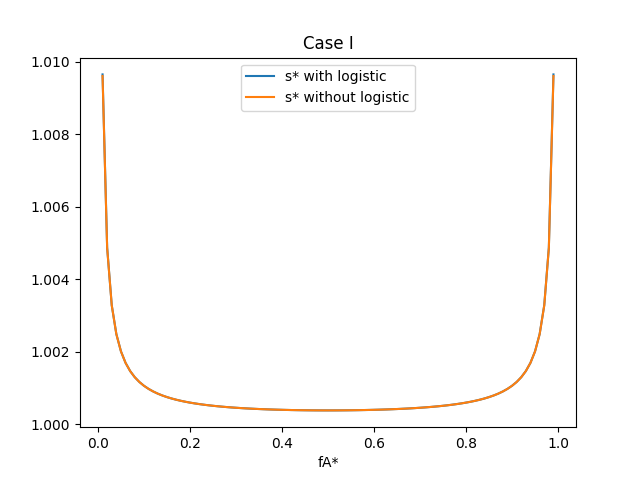
\includegraphics[width=\linewidth]{sstar_caseI}
%	\caption{}\label{fig:awes}
%	\endminipage\hfill
%	\minipage{0.25\textwidth}
%	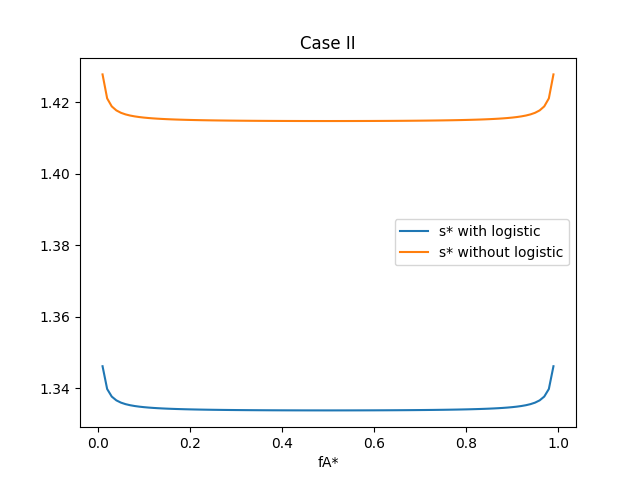
\includegraphics[width=\linewidth]{sstar_caseII}
%	\caption{}\label{fig:awesome_image2}
%	\endminipage\hfill
%	\minipage{0.25\textwidth}%
%	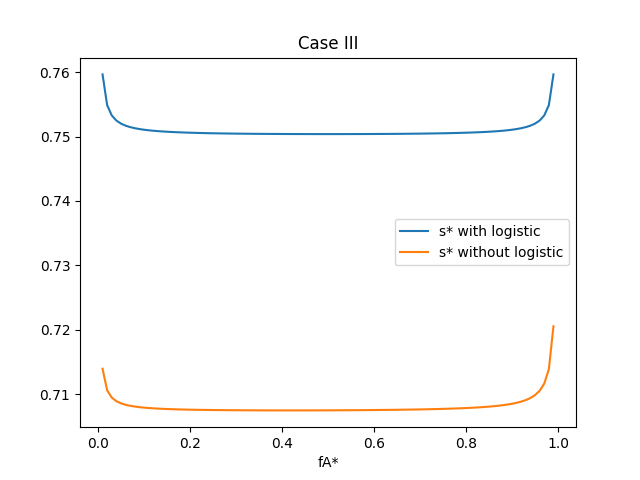
\includegraphics[width=\linewidth]{sstar_caseIII}
%	\caption{}\label{fig:awesome_image3}
%	\endminipage
%		\minipage{0.25\textwidth}%
%	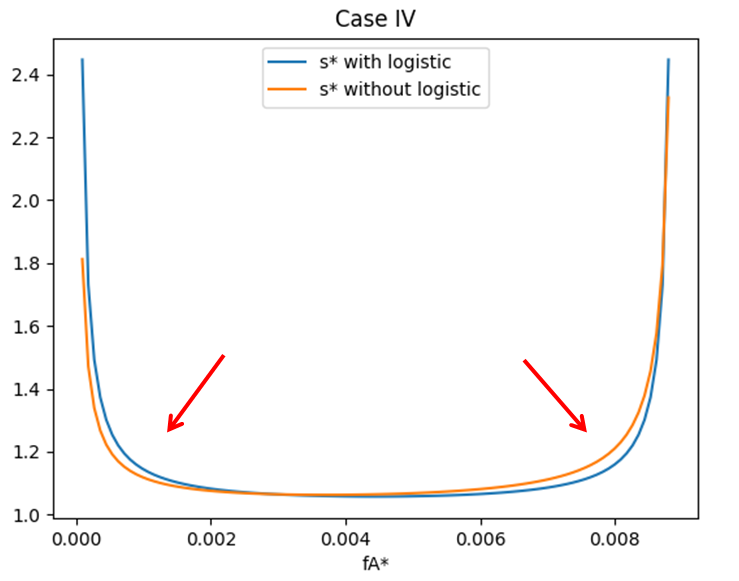
\includegraphics[width=0.9\linewidth]{caseIVmodi}
%	\caption{}\label{fig:awesome_image3}
%	\endminipage
%	
%\end{figure}






\begin{figure}
%	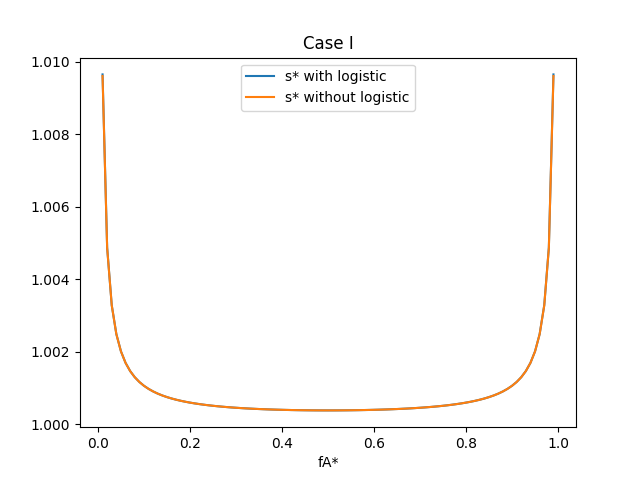
\includegraphics[width=3.2cm]{sstar_caseI}
%	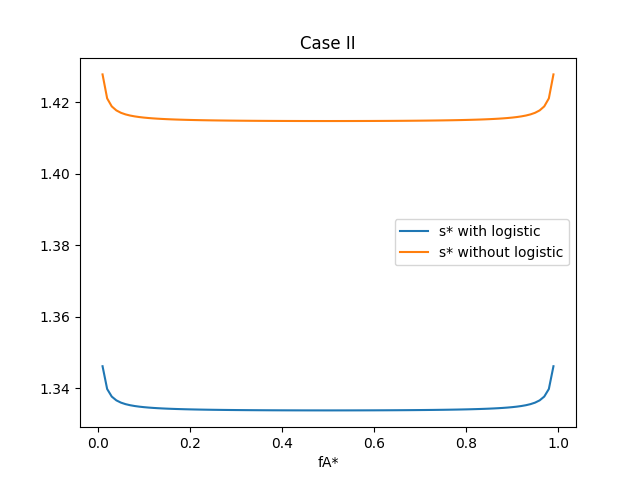
\includegraphics[width=3.2cm]{sstar_caseII}
%	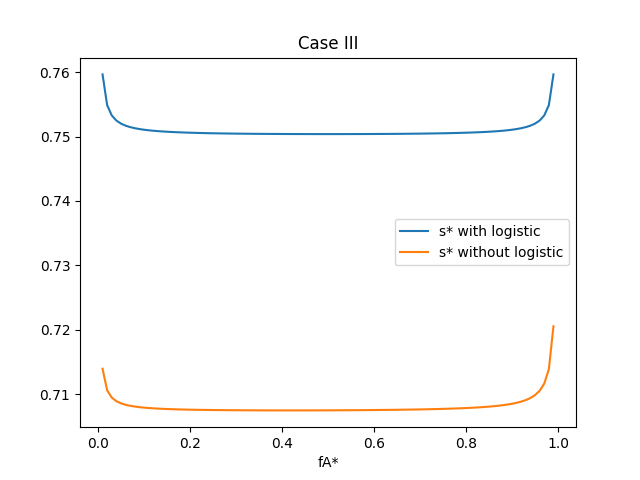
\includegraphics[width=3.2cm]{sstar_caseIII}
%	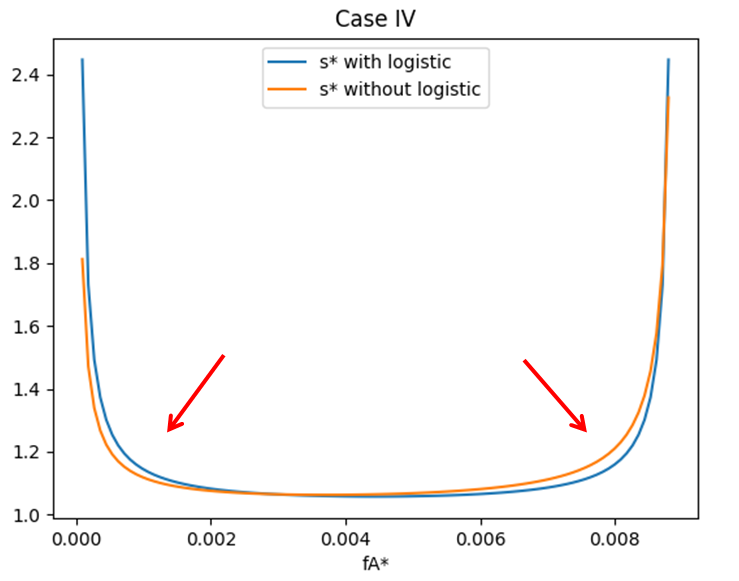
\includegraphics[width=2.9cm]{caseIVmodi}

%	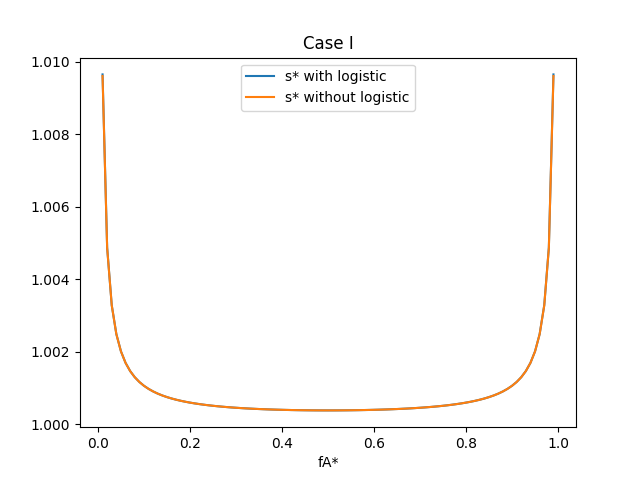
\includegraphics[width=3.2cm]{sstar_caseI}
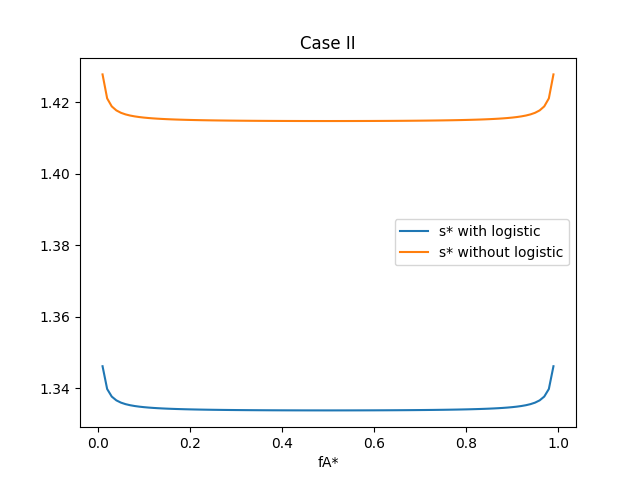
\includegraphics[width=4cm]{sstar_caseII}
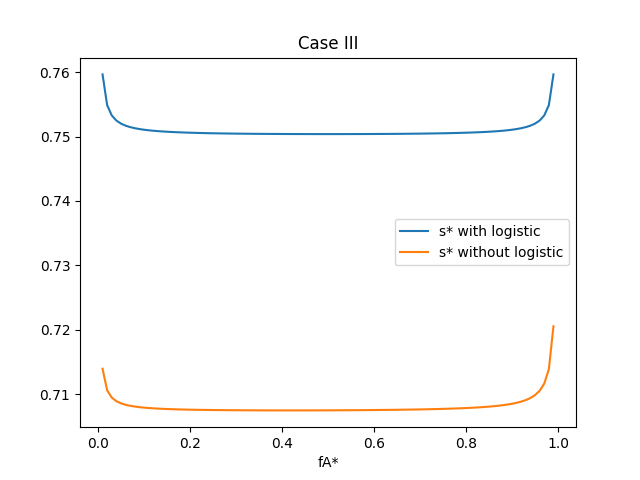
\includegraphics[width=4cm]{sstar_caseIII}
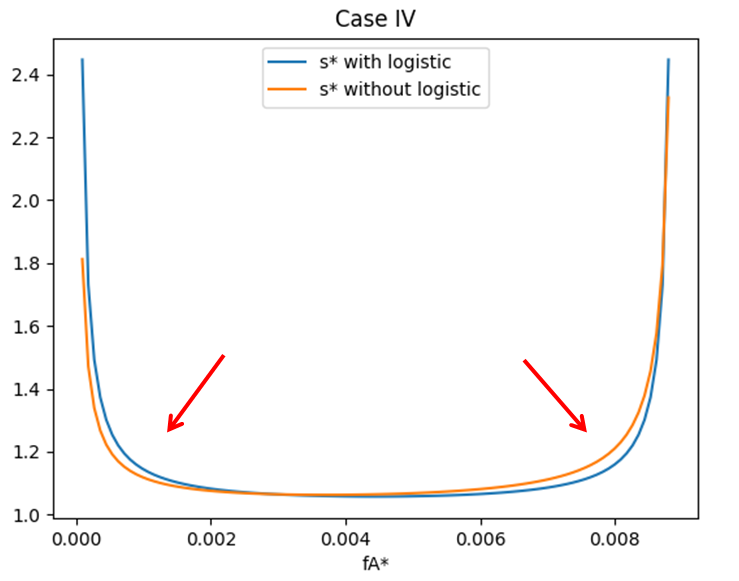
\includegraphics[width=3.9cm]{caseIVmodi}

\end{figure}






\end{frame}




\begin{frame}
\frametitle{Numerical simulations}
\end{frame}


\begin{frame}
\frametitle{Numerical simulations}
\begin{columns}[T] % align columns
	\begin{column}{.48\textwidth}
		\color{orange}\rule{\linewidth}{4pt}
		
		Micro
	\end{column}%
	\hfill%
	\begin{column}{.48\textwidth}
		\color{blue}\rule{\linewidth}{4pt}
		
		Macro
	\end{column}%
\end{columns}
\end{frame}

\begin{frame}
\frametitle{blabla}
\end{frame}




\section{Any questions?}
\begin{frame}
\frametitle{Thank you!}
%%\begin{figure}[h]
%%\centering
%%\includegraphics[scale=.2,keepaspectratio]{}
%%\end{figure}
\end{frame}





\end{document}

